\begin{figure}
\centering
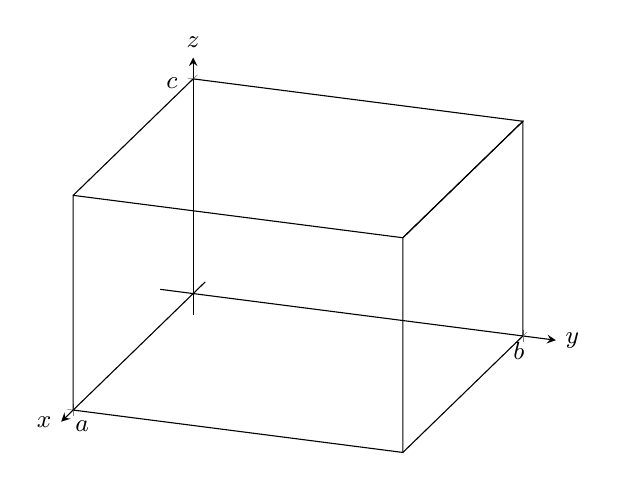
\begin{tikzpicture}[font=\small,]
\pgfmathsetmacro{\a}{1.5}
\pgfmathsetmacro{\b}{2}
\pgfmathsetmacro{\c}{1}
\begin{axis}[clip=false,axis lines=center,view/h=110,enlargelimits=true,xtick={\a},ytick={\b},ztick={\c},xticklabels={$a$},yticklabels={$b$},zticklabels={$c$},xlabel={$x$},ylabel={$y$},zlabel={$z$},xlabel style={anchor=east},ylabel style={anchor=west},zlabel style={anchor=south}]
\addplot3[]coordinates{(\a,0,0)(\a,\b,0)(\a,\b,\c)(\a,0,\c)(\a,0,0)};
\addplot3[]coordinates{(\a,\b,0)(0,\b,0)(0,\b,\c)(\a,\b,\c)};
\addplot3[]coordinates{(\a,0,\c)(0,0,\c)(0,\b,\c)(\a,\b,\c)};
\end{axis}
\end{tikzpicture}
\end{figure}

\begin{figure}
\centering
\begin{tikzpicture}[font=\small,]
\pgfmathsetmacro{\a}{1.5}
\pgfmathsetmacro{\b}{2}
\pgfmathsetmacro{\c}{1}
\begin{axis}[clip=false,axis lines=center,view/h=110,enlargelimits=true,xtick={\a},ytick={\b},ztick={\c},xticklabels={$a$},yticklabels={$b$},zticklabels={$c$},xlabel={$x$},ylabel={$y$},zlabel={$z$},xlabel style={anchor=east},ylabel style={anchor=west},zlabel style={anchor=south}, hide axis]
\addplot3[]coordinates{(1/2*\a,-1/3*\b,-1/3*\c)(1/2*\a,2/3*\b,-1/3*\c)(1/2*\a,-1/3*\b,2/3*\c)(1/2*\a,-1/3*\b,-1/3*\c)};
\addplot3[]coordinates{(1/2*\a,2/3*\b,-1/3*\c)(-1/2*\a,2/3*\b,-1/3*\c)(-1/2*\a,-1/3*\b,2/3*\c)(1/2*\a,-1/3*\b,2/3*\c)};
\addplot3[-latex]coordinates{(1/2*\a,0,0)(1.75*\a,0,0)}node[below]{$x$};
\addplot3[-latex]coordinates{(0,1/3*\b,0)(0,\b,0)}node[right]{$y$};
\addplot3[-latex]coordinates{(0,0,1/3*\c)(0,0,\c)}node[above]{$z$};
\addplot3[stealth-stealth]coordinates{(1/2*\a,0,-1/3*\c)(1/2*\a,0,0)}node[pos=0.5,right]{$\tfrac{c}{3}$};
\addplot3[stealth-stealth]coordinates{(1/2*\a,0,0)(1/2*\a,-1/3*\b,0)}node[pos=0.5,above]{$\tfrac{b}{3}$};
\addplot3[stealth-stealth]coordinates{(0,0,1/3*\c)(1/2*\a,0,1/3*\c)}node[pos=0.5,above left]{$\tfrac{a}{2}$};
\addplot3[]coordinates{(1/2*\a,1/3*\b,-1/3*\c)}node[below]{$b$};
\addplot3[]coordinates{(0,2/3*\b,-1/3*\c)}node[right]{$a$};
\addplot3[]coordinates{(1/2*\a,-1/3*\b,1/3*\c)}node[left]{$c$};
\addplot3[]coordinates{(-1/2*\a,1/3*\b,1/3*\c)}node[above,align=center]{\text{\RL{وسطانی مرکز}}\\  \عددی{(0,0,0)}};
\end{axis}
\end{tikzpicture}
\end{figure}


\begin{figure}
\centering
\begin{tikzpicture}[font=\small,declare function={fx(\r,\t)=2*\r*cos(\t);fy(\r,\t)=\r*sin(\t);fz(\r,\t)=2-2*\r*cos(\t);}]
\pgfmathsetmacro{\ta}{160}
\begin{axis}[clip=false,axis lines=center,view/h=160,enlargelimits=true,xlabel={$x$},ylabel={$y$},zlabel={$z$},xlabel style={anchor=east},ylabel style={anchor=west},zlabel style={anchor=south},xtick={\empty},ytick={\empty},ztick={\empty},hide axis]
\addplot3[smooth,domain y=0:360,variable y=\t] ({fx(1,t)},{fy(1,t)},{fz(1,t)})node[pos=0.75,pin=135:{$z=2-x$}]{};
\addplot3[smooth,domain y=0:360,variable y=\t] ({fx(1,t)},{fy(1,t)},0)node[pos=0.4,pin=-45:{$x^2+4y^2=4$}]{};
\addplot3[]coordinates{({fx(1,\ta)},{fy(1,\ta)},{fz(1,\ta)}) ({fx(1,\ta)},{fy(1,\ta)},0)};
\addplot3[dashed]coordinates{(0,0,0)(2,0,0)}node[circ]{}node[below]{$2$};
\addplot3[-latex]coordinates{(2,0,0)(2.5,0,0)}node[left]{$x$};
\addplot3[dashed]coordinates{(0,0,0)(0,1,0)}node[circ]{}node[below]{$1$};
\addplot3[-latex]coordinates{(0,1,0)(0,2,0)}node[right]{$y$};
\addplot3[dashed]coordinates{(0,0,0)(0,0,2)}node[circ]{}node[left]{$2$};
\addplot3[-latex]coordinates{(0,0,2)(0,0,4.5)}node[left]{$z$};
\end{axis}
\end{tikzpicture}
\end{figure}


\begin{figure}
\centering
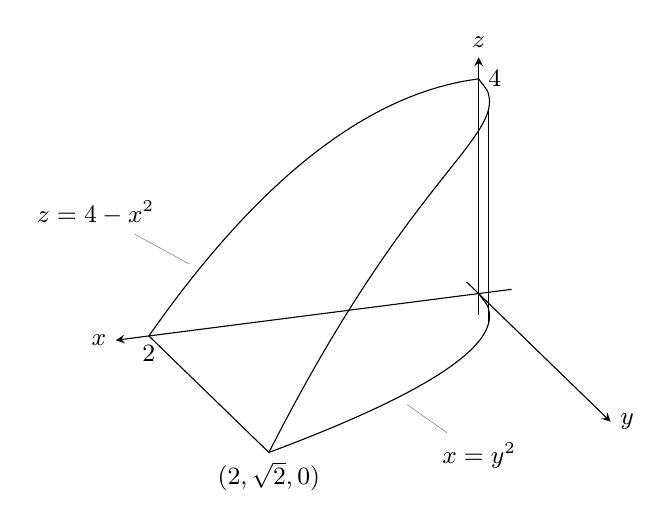
\begin{tikzpicture}[font=\small,declare function={fx(\x)=\x;fy(\x)=sqrt(\x);fz(\x)=4-(\x)^2;}]
\pgfmathsetmacro{\xa}{0.4}
\pgfmathsetmacro{\xb}{0.1}
\begin{axis}[clip=false,axis lines=center,view/h=160,enlargelimits=true,xlabel={$x$},ylabel={$y$},zlabel={$z$},xlabel style={anchor=east},ylabel style={anchor=west},zlabel style={anchor=south},xtick={\empty},ytick={\empty},ztick={\empty}]
\addplot3[smooth,domain=0:\xa,samples y=0] ({fx(x)},{fy(x)},{fz(x)});
\addplot3[smooth,domain=0:\xa,samples y=0] ({fx(x)},{fy(x)},0);
\addplot3[smooth,domain=\xa:2,samples y=0] ({fx(x)},{fy(x)},{fz(x)});
\addplot3[smooth,domain=\xa:2,samples y=0] ({fx(x)},{fy(x)},0)node[pos=0.4,pin=-45:{$x=y^2$}]{};
\addplot3[smooth,domain=0:2,samples y=0] ({fx(x)},0,{fz(x)})node[pos=0.75,pin=135:{$z=4-x^2$}]{};
\addplot3[]coordinates{(2,0,0)(2,sqrt(2),0)}node[pos=0,below]{$2$}node[below]{$(2,\sqrt{2},0)$};
\addplot3[]coordinates{ ({fx(\xb)},{fy(\xb)},{fz(\xb)}) ({fx(\xb)},{fy(\xb)},0)};
\addplot3[]coordinates{(0,0,4)}node[right]{$4$};
\end{axis}
\end{tikzpicture}
\end{figure}

\begin{figure}
\centering
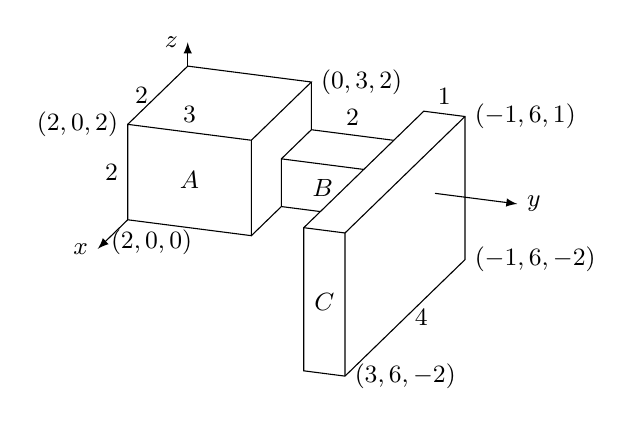
\begin{tikzpicture}[font=\small,declare function={fx(\x)=\x;fy(\x)=sqrt(\x);fz(\x)=4-(\x)^2;}]
\pgfmathsetmacro{\xa}{0.4}
\pgfmathsetmacro{\xb}{0.1}
\begin{axis}[clip=false,axis lines=center,view/h=110,enlargelimits=true,xlabel={$x$},ylabel={$y$},zlabel={$z$},xlabel style={anchor=east},ylabel style={anchor=west},zlabel style={anchor=south},xtick={\empty},ytick={\empty},ztick={\empty},hide axis]
\addplot3[]coordinates{(2,0,0)(2,3,0)(2,3,2)(2,0,2)(2,0,0)};
\addplot3[]coordinates{(2,3,2)(0,3,2)(0,0,2)(2,0,2)};
\addplot3[]coordinates{(2,3,0) (1,3,0) (1,3,1)(0,3,1) (0,3,2)};
\addplot3[]coordinates{(1,3,0)(1,5,0)};
\addplot3[]coordinates{(1,3,1)(1,5,1)};
\addplot3[]coordinates{(0,3,1)(0,5,1)};
\addplot3[fill=white]coordinates{(3,6,-2)(-1,6,-2)(-1,6,1)(-1,5,1)(3,5,1)(3,5,-2)(3,6,-2)};
\addplot3[]coordinates{(3,6,-2)(3,6,1)(-1,6,1)};
\addplot3[]coordinates{(3,5,1)(3,6,1)};
\addplot3[-latex]coordinates{(2,0,0)(3,0,0)}node[left]{$x$};
\addplot3[-latex]coordinates{(0,6,0)(0,8,0)}node[right]{$y$};
\addplot3[-latex]coordinates{(0,0,2)(0,0,2.5)}node[left]{$z$};
\addplot3[]coordinates{(2,0,2)}node[left]{$(2,0,2)$};
\addplot3[]coordinates{(2,0,0)}node[below,xshift=2ex]{$(2,0,0)$};
\addplot3[]coordinates{(3,6,-2)}node[right]{$(3,6,-2)$};
\addplot3[]coordinates{(-1,6,-2)}node[right]{$(-1,6,-2)$};
\addplot3[]coordinates{(-1,6,1)}node[right]{$(-1,6,1)$};
\addplot3[]coordinates{(0,3,2)}node[right]{$(0,3,2)$};
\addplot3[]coordinates{(-1,5.5,1)}node[above]{$1$};
\addplot3[]coordinates{(0,4,1)}node[above]{$2$};
\addplot3[]coordinates{(1,0,2)}node[left]{$2$};
\addplot3[]coordinates{(2,1.5,2)}node[above]{$3$};
\addplot3[]coordinates{(2,0,1)}node[left]{$2$};
\addplot3[]coordinates{(1,6,-2)}node[right]{$4$};
\addplot3[]coordinates{(2,1.5,1)}node[]{$A$};
\addplot3[]coordinates{(1,4,0.5)}node[]{$B$};
\addplot3[]coordinates{(3,5.5,-0.5)}node[]{$C$};
\end{axis}
\end{tikzpicture}
\end{figure}




\begin{figure}
\centering
\begin{tikzpicture}[font=\small,declare function={fx(\x)=cos(\x);fy(\x)=sin(\x);}]
\pgfmathsetmacro{\xa}{135}
\pgfmathsetmacro{\xb}{\xa+180}
\pgfmathsetmacro{\xc}{65}
\pgfmathsetmacro{\xd}{\xc+180}
\pgfmathsetmacro{\a}{1.5}
\pgfmathsetmacro{\b}{1.25}
\begin{axis}[clip=false,axis lines=center,view/h=135,enlargelimits=true,xlabel={$x$},ylabel={$y$},zlabel={$z$},xlabel style={anchor=east},ylabel style={anchor=west},zlabel style={anchor=south},xtick={\empty},ytick={\empty},ztick={\empty},hide  axis]
\addplot3[domain=0:360]({fx(x)},{fy(x)},2);
\addplot3[domain=0:360]({fx(x)},{fy(x)},0);
\addplot3[]coordinates{({fx(\xa)},{fy(\xa)},{2})({fx(\xa)},{fy(\xa)},0)};
\addplot3[]coordinates{({fx(\xb)},{fy(\xb)},{2})({fx(\xb)},{fy(\xb)},0)};
\addplot3[]coordinates{(-\a,-\b,2)(\a,-\b,2)(\a,\b,2)(-\a,\b,2)(-\a,-\b,2)};
\addplot3[]coordinates{({2*fx(\xc)},{2*fy(\xc)},2)({2*fx(\xc)},{2*fy(\xc)},0)({2*fx(\xd)},{2*fy(\xd)},0)({2*fx(\xd)},{2*fy(\xd)},2) ({2*fx(\xc)},{2*fy(\xc)},2)};
\addplot3[thick]coordinates{({fx(\xc)},{fy(\xc)},0)({fx(\xc)},{fy(\xc)},2)}node[circ]{}node[pin={[pin distance=1cm,right]-10:{$(\rho,\phi,z)$}}]{};
\addplot3[-stealth,domain=0:\xc,samples y=0] ({1.2*fx(x)},{1.2*fy(x)},0)node[pos=0.4,below]{$\phi$};
\addplot3[thick]coordinates{(0,0,0)({fx(\xc)},{fy(\xc)},0)}node[pos=0.6,left]{$\rho$};
\addplot3[dashed]coordinates{(0,0,0)(0,0,2)}node[circ]{}node[right]{$z$};
\addplot3[-latex]coordinates{(0,0,2)(0,0,3.5)}node[left]{$z$};
\addplot3[-latex]coordinates{(0,0,0)(2,0,0)}node[left]{$x$};
\addplot3[-latex]coordinates{(0,0,0)(0,2,0)}node[right]{$y$};
\end{axis}
\end{tikzpicture}
\end{figure}


\begin{figure}
\centering
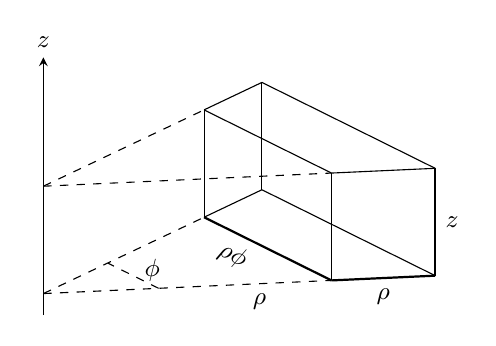
\begin{tikzpicture}[font=\small,declare function={fx(\r,\t)=\r*cos(\t);fy(\r,\t)=\r*sin(\t);}]
\pgfmathsetmacro{\ta}{30}
\pgfmathsetmacro{\tb}{\ta+45}
\pgfmathsetmacro{\ra}{1.25}
\pgfmathsetmacro{\rb}{\ra+0.45}
\pgfmathsetmacro{\h}{0.5}
\begin{axis}[clip=false,axis lines=center,view/h=20,enlargelimits=true,xlabel={$x$},ylabel={$y$},zlabel={$z$},xlabel style={anchor=east},ylabel style={anchor=west},zlabel style={anchor=south},xtick={\empty},ytick={\empty},ztick={\empty},xmin=0,ymin=0,zmin=0,zmax=1,hide x axis, hide y axis]
\addplot3[thick,domain y=\ta:\tb,samples=0,variable=\r,variable y=\t] ({fx(\ra,t)},{fy(\ra,t)},0)node[pos=0.7,sloped,below]{$\rho\dif\phi$};
\addplot3[domain y=\ta:\tb,samples=0,variable=\r,variable y=\t] ({fx(\rb,t)},{fy(\rb,t)},0);
\addplot3[domain y=\ta:\tb,samples=0,variable=\r,variable y=\t] ({fx(\ra,t)},{fy(\ra,t)},\h);
\addplot3[domain y=\ta:\tb,samples=0,variable=\r,variable y=\t] ({fx(\rb,t)},{fy(\rb,t)},\h);
\addplot3[thick]coordinates{({fx(\ra,\ta)},{fy(\ra,\ta)},0)({fx(\rb,\ta)},{fy(\rb,\ta)},0)}node[pos=0.5,below]{$\dif\rho$};
\addplot3[]coordinates{({fx(\ra,\tb)},{fy(\ra,\tb)},0)({fx(\rb,\tb)},{fy(\rb,\tb)},0)};
\addplot3[]coordinates{({fx(\ra,\ta)},{fy(\ra,\ta)},\h)({fx(\rb,\ta)},{fy(\rb,\ta)},\h)};
\addplot3[]coordinates{({fx(\ra,\tb)},{fy(\ra,\tb)},\h)({fx(\rb,\tb)},{fy(\rb,\tb)},\h)};
\addplot3[]coordinates{({fx(\ra,\ta)},{fy(\ra,\ta)},0)({fx(\ra,\ta)},{fy(\ra,\ta)},\h)};
\addplot3[thick]coordinates{({fx(\rb,\ta)},{fy(\rb,\ta)},0)({fx(\rb,\ta)},{fy(\rb,\ta)},\h)}node[pos=0.5,right]{$\dif z$};
\addplot3[]coordinates{({fx(\ra,\tb)},{fy(\ra,\tb)},0)({fx(\ra,\tb)},{fy(\ra,\tb)},\h)};
\addplot3[]coordinates{({fx(\rb,\tb)},{fy(\rb,\tb)},0)({fx(\rb,\tb)},{fy(\rb,\tb)},\h)};
\addplot3[dashed]coordinates{(0,0,0)({fx(\ra,\ta)},{fy(\ra,\ta)},0)}node[pos=0.75,below]{$\rho$};
\addplot3[dashed]coordinates{(0,0,0)({fx(\ra,\tb)},{fy(\ra,\tb)},0)};
\addplot3[dashed]coordinates{(0,0,\h)({fx(\ra,\ta)},{fy(\ra,\ta)},\h)};
\addplot3[dashed]coordinates{(0,0,\h)({fx(\ra,\tb)},{fy(\ra,\tb)},\h)};
\addplot3[dashed,samples=0,domain y=\ta:\tb,variable y=\t]({fx(0.5,t)},{fy(0.5,t)},0)node[pos=0.7,xshift=1ex,right]{$\dif \phi$};
\end{axis}
\end{tikzpicture}
\end{figure}


\begin{figure}
\centering
\begin{tikzpicture}[font=\small,declare function={fx(\x)=cos(\x);fy(\x)=1+sin(\x);fz(\x)=2+2*sin(\x);}]
\pgfmathsetmacro{\xa}{110}
\pgfmathsetmacro{\xb}{\xa+180}
\pgfmathsetmacro{\xx}{0.35}
\pgfmathsetmacro{\yy}{1.7}
\pgfmathsetmacro{\yyy}{2.5}
\pgfmathsetmacro{\zz}{4}
\pgfmathsetmacro{\angL}{atan(\yy/\xx)}
\begin{axis}[clip=false,axis lines=center,view/h=110,enlargelimits=true,xlabel={$x$},ylabel={$y$},zlabel={$z$},xlabel style={anchor=east},ylabel style={anchor=west},zlabel style={anchor=south},xtick={\empty},ytick={2},ztick={\empty},zmax=5,hide z axis]
\addplot3[domain=0:360]({fx(x)},{fy(x)},{fz(x)})node[pos=0.9,pin={[font=\scriptsize]135:{\begin{minipage}{2cm} \begin{align*} z&=x^2+y^2 &&\text{کارتیسی}\\ z&=\rho^2&&\text{نلکی}\end{align*} \end{minipage}}}]{};
\addplot3[domain=0:360]({fx(x)},{fy(x)},0)node[pos=0.195,below]{$R$}node[pos=0.2,pin={[font=\scriptsize]-45:{\begin{minipage}{2cm} \begin{align*}&x^2+(y-1)^2=1&&\text{کارتیسی}\\ &\rho=2\sin\phi &&\text{نلکی} \end{align*}\end{minipage}}}]{};
\addplot3[] coordinates{({fx(\xa)},{fy(\xa)},{fz(\xa)})({fx(\xa)},{fy(\xa)},0)}node[pos=0.5,right]{$D$};
\addplot3[] coordinates{({fx(\xb)},{fy(\xb)},{fz(\xb)})({fx(\xb)},{fy(\xb)},0)};
\addplot3[dashed]coordinates{(\xx,\yy,0)(\xx,\yy,\zz)}node[pos=0,pin=-45:{$(\rho,\phi)$}]{}node[pos=0,circ]{}node[pos=1,circ]{};
\addplot3[-latex]coordinates{(\xx,\yy,\zz)(\xx,\yy,6)}node[right]{$M$};
\addplot3[-latex]coordinates{(0,0,0)(\xx*\yyy/\yy,\yyy,0)}node[right]{$L$};
\addplot3[-latex]coordinates{(0,0,0)(0,0,2)}node[left]{$z$};
\addplot3[-stealth,domain=0:\angL,samples y=0]({0.6*cos(x)},{0.6*sin(x)},0)node[pos=0.75,below]{$\phi$};
\end{axis}
\end{tikzpicture}
\end{figure}


\begin{figure}
\centering
\begin{tikzpicture}[font=\small]
\pgfmathsetmacro{\ang}{atan(0.25/0.5)}
\pgfmathsetmacro{\a}{1}
\pgfmathsetmacro{\b}{0.75*\a}
\pgfmathsetmacro{\h}{2}
\draw(0,0) circle (\a cm and \b cm);
\draw(0,\h) circle (\a cm and \b cm);
\draw[]plot [domain=-1:1] (\x,{2*(\x)^2});
\draw(-0.75,{2*(0.75)^2})node[pin={-135:{$\begin{aligned}z&=x^2+y^2\\  z&=\rho^2\end{aligned}$}}]{};
\draw(-\a,0)--++(0,\h);
\draw(\a,0)--++(0,\h)node[pos=0.5,pin=45:{$\begin{aligned}x^2+y^2&=4\\  \rho&=2  \end{aligned}$}]{};
\draw(0.5,-0.25)node[circ]{}node[pin=-80:{$(\rho,\phi)$}]{}--++(0,1.25)node[circ]{};
\path[name path=klid]([shift={(180:\a cm and \b cm)}]0,\h) arc (180:360:\a cm and \b cm);
\path[name path=kM] (0.5,-0.25)++(0,1.25)--++(0,1);
\draw[-latex,name intersections={of={kM and klid}}](intersection-1)--++(0,0.5)node[above]{$M$};
\draw[-latex](0,0)--(1.25,-1.25*0.25/0.5)node[right]{$L$};
\draw[-latex](0,0)--++(-135:1.2)node[left]{$x$};
\draw[-latex](0,0)--++(2,0)node[right]{$y$};
\draw[-latex](0,\h-\b)--++(0,2)node[left]{$z$};
\draw(0,\h)node[left]{$4$}--++(0.1,0);
\draw[-stealth]([shift={(-135:0.3)}]0,0) arc (-135:-\ang:0.3)node[pos=0.6,below]{$\phi$};
\end{tikzpicture}
\end{figure}


 \begin{figure}
\centering
\begin{subfigure}{0.30\textwidth}
\centering
\begin{tikzpicture}[font=\scriptsize]
\pgfmathsetmacro{\angA}{-170}
\pgfmathsetmacro{\angB}{100}
\pgfmathsetmacro{\angC}{-10}
\pgfmathsetmacro{\angD}{-135}
\pgfmathsetmacro{\angE}{-100}
\pgfmathsetmacro{\angF}{-40}
\draw[-latex,name path=kx](0,0)--++(-1.5,-1.5)node[right]{$x$};
\draw[-latex](0,0)--++(2.5,0)node[right]{$y$};
\draw[-latex](0,0)--++(0,2)node[left]{$z$};
\draw[fill=lgray,draw=black,text=black,opacity=0.5](2.25,-0.25)coordinate(kA) to [out=\angA,in=\angB]node[pos=0.75,above left,yshift=-1ex,font=\scriptsize]{$\rho=h_1(\phi)$}++(-1.5,-0.75)coordinate(kB)node[above right,xshift=1ex,yshift=0.5ex]{$R$} to [out=\angC,in=\angD]node[pos=0.5,right]{$\rho=h_2(\phi)$}(kA);
\path[dashed](kA)--++(0,2.25)coordinate(kC)coordinate[pos=0.5](kE);
\path[dashed](kB)--++(0,3)coordinate(kD)coordinate[pos=0.5](kF);
\draw[dashed](kA)--(kE)  (kB)--(kF);
\draw(kC)--(kE)  (kD)--(kF);
\draw[dashed](kE) to [out=\angA,in=\angB](kF);
\draw(kF) to [out=\angC,in=\angD](kE); 
\draw(kE) to [out=\angE,in=\angF]coordinate[pos=0.25](kLower)(kF);
\draw(kC) to [out=110,in=60]coordinate[pos=0.25](kUpper)(kD);
\draw[](kC) to [out=-\angA,in=-\angB](kD);
\draw[dashed](kD) to [out=-\angC,in=-\angD](kC);
\draw(kLower)node[pin={[right,pin distance=0.25cm,font=\scriptsize]10:{$z=g_1(\rho,\phi)$}}]{};
\draw(kUpper)node[pin={[above]35:{$z=g_2(\rho,\phi)$}}]{};
\draw($(kC)!0.5!(kE)$)node[right]{$D$};
\end{tikzpicture}
\caption{}
\end{subfigure}\hfill
\begin{subfigure}{0.30\textwidth}
\centering
\begin{tikzpicture}[font=\scriptsize]
\pgfmathsetmacro{\angA}{-170}
\pgfmathsetmacro{\angB}{100}
\pgfmathsetmacro{\angC}{-10}
\pgfmathsetmacro{\angD}{-135}
\pgfmathsetmacro{\angE}{-100}
\pgfmathsetmacro{\angF}{-40}
\draw[-latex,name path=kx](0,0)--++(-1.5,-1.5)node[right]{$x$};
\draw[-latex](0,0)--++(2.5,0)node[right]{$y$};
\draw[-latex](0,0)--++(0,2)node[left]{$z$};
\draw[fill=lgray,draw=black,text=black,opacity=0.5](2.25,-0.25)coordinate(kA) to [out=\angA,in=\angB]node[pos=0.5, left,xshift=-2ex,yshift=-1ex,font=\scriptsize]{$\rho=h_1(\phi)$}++(-1.5,-0.75)coordinate(kB)node[above right,xshift=1ex,yshift=0.5ex]{$R$} to [out=\angC,in=\angD]node[pos=0.75,right,font=\scriptsize]{$\rho=h_2(\phi)$}(kA);
\path[dashed](kA)--++(0,2.25)coordinate(kC)coordinate[pos=0.5](kE);
\path[dashed](kB)--++(0,3)coordinate(kD)coordinate[pos=0.5](kF);
%\draw[dashed](kA)--(kE)  (kB)--(kF);
\draw(kC)--(kE)  (kD)--(kF);
\draw[dashed](kE) to [out=\angA,in=\angB](kF);
\draw(kF) to [out=\angC,in=\angD](kE); 
\draw(kE) to [out=\angE,in=\angF]coordinate[pos=0.25](kLower)(kF);
\draw(kC) to [out=110,in=60]coordinate[pos=0.25](kUpper)(kD);
\draw[](kC) to [out=-\angA,in=-\angB](kD);
\draw[dashed](kD) to [out=-\angC,in=-\angD](kC);
\draw($(kC)!0.5!(kE)$)node[right]{$D$};
\draw($(kA)!0.5!(kB)$)node[circ]{}node[pin={[pin distance=0.25cm]-45:{$(\rho,\phi)$}}]{}--($(kE)!0.5!(kF)+(0,-0.3)$)coordinate(kMm)node[circ]{};
\draw[dashed](kMm)node[pin={[right,pin edge={-,solid},align=center,pin distance=1cm]30:{\text{\RL{داخل}}\\ $z=g_1(\rho,\phi)$}}]{}--($(kC)!0.5!(kD)$)node[circ]{}node[pin={[align=center,pin edge={-,solid}]35:{\text{\RL{خارج}}\\ $z=g_2(\rho,\phi)$}}]{};
\draw[-latex]($(kC)!0.5!(kD)$)--++(0,1)node[left]{$M$};
\end{tikzpicture}
\caption{}
\end{subfigure}\hfill
\begin{subfigure}{0.30\textwidth}
\centering
\begin{tikzpicture}[font=\scriptsize]
\pgfmathsetmacro{\angA}{-170}
\pgfmathsetmacro{\angB}{100}
\pgfmathsetmacro{\angC}{-10}
\pgfmathsetmacro{\angD}{-135}
\pgfmathsetmacro{\angE}{-100}
\pgfmathsetmacro{\angF}{-40}
\pgfmathsetmacro{\angMM}{atan(-0.625/1.55)}
\pgfmathsetmacro{\angEE}{atan(-0.25/2.25)}
\pgfmathsetmacro{\angSS}{atan(-1/0.75)}
\draw[-latex,name path=kx](0,0)--++(-1.5,-1.5)node[right]{$x$};
\draw[-latex](0,0)--++(2.25,0)node[right]{$y$};
\draw[-latex](0,0)--++(0,2)node[left]{$z$};
\draw[fill=lgray,draw=black,text=black,opacity=0.5](2.25,-0.25)coordinate(kA)node[circ]{} to [out=\angA,in=\angB]++(-1.5,-0.75)coordinate(kB)node[circ]{}node[right,xshift=2ex,yshift=-1ex]{$R$} to [out=\angC,in=\angD](kA);
\path[name path=kR](kA) to [out=\angA,in=\angB](kB);
\path[name path=kL](kB) to [out=\angC,in=\angD](kA);
\path[dashed](kA)--++(0,2.25)coordinate(kC)coordinate[pos=0.5](kE);
\path[dashed](kB)--++(0,3)coordinate(kD)coordinate[pos=0.5](kF);
\draw(kC)--(kE)  (kD)--(kF);
\draw[dashed](kE) to [out=\angA,in=\angB](kF);
\draw(kF) to [out=\angC,in=\angD](kE); 
\draw(kE) to [out=\angE,in=\angF]coordinate[pos=0.25](kLower)(kF);
\draw(kC) to [out=110,in=60]coordinate[pos=0.25](kUpper)(kD);
\draw[](kC) to [out=-\angA,in=-\angB](kD);
\draw[dashed](kD) to [out=-\angC,in=-\angD](kC);
\draw($(kC)!0.5!(kE)$)node[right]{$D$};
\draw($(kA)!0.5!(kB)$)coordinate(kLM)node[circ]{}node[xshift=-2ex,yshift=-1ex]{$(\rho,\phi)$}--($(kE)!0.5!(kF)+(0,-0.3)$)coordinate(kMm)node[circ]{};
\draw[dashed](kMm)--($(kC)!0.5!(kD)$)node[circ]{};
\draw[-latex]($(kC)!0.5!(kD)$)--++(0,1)node[left]{$M$};
\draw[-latex,name path=kray](0,0)--++(\angMM:2.25)node[right]{$L$};
\draw[name intersections={of=kR and kray}](intersection-1)node[circ]{}node[pin={[align=center,pin distance=0.75cm]-170:{\text{داخل}\\$\rho=h_1(\phi)$}}]{};
\draw[name intersections={of=kL and kray}](intersection-1)node[circ]{}node[pin={[align=center,pin distance=0.25cm,below]-70:{\text{خارج}\\  $\rho=h_2(\phi)$}}]{};
\draw[-latex](0,0)--++(\angEE:2.75)node[right]{$\phi=\beta$};
\draw[-latex](0,0)--++(\angSS:1.75)node[left,yshift=-1ex]{$\phi=\alpha$};
\draw[-stealth]([shift={(-135:0.3)}]0,0) arc (-135:\angSS:0.3)node[pos=0.5,below]{$\alpha$};
\end{tikzpicture}
\caption{}
\end{subfigure}
\end{figure}

